\documentclass[10pt,letterpaper,conference]{IEEEtran}

\usepackage{cite}
\usepackage{amsmath}
\usepackage{comment}
%\usepackage{times}
\usepackage{epsfig}
\usepackage{url}
\usepackage{multirow}

\textheight 688pt

\begin{document}
\title{Device-Architecture Co-Optimization of STT-RAM Caches for Embedded Applications\vspace{-10pt}}
%\author{Cong Xu\dag, Xiaochun Zhu\dag\ddag, Dimin Niu\dag, Yuan Xie\dag, Seung H. Kang\dag\ddag\\
%\dag Department of Computer Science and Engineering, Pennsylvania State University\\
%\ddag Emerging Memory Technology Group, Qualcomm Incorpotation\vspace{-15pt}}

\maketitle

\begin{abstract}

Spin-transfer torque random access memory (STT-RAM) is a fast, scalable, durable non-volatile memory which can be embedded into standard CMOS process. A wide range of write speeds from $1ns$ to $100ns$ have been reported for STT-RAM. The switching current of magnetic tunnel junction (MTJ) that is the basic building block of STT-RAM is inversely proportional to the write pulse width. In this work, we provide a detailed methodology to design STT-RAM for different optimization goals such as read performance, write performance and write energy by leveraging the trade-off between write current and write time of MTJ. We take the typical in-plane MTJ and advanced perpendicular MTJ (PMTJ) as our optimization targets. Our study shows that the reducing write pulse width will harm read latency and energy. While "sweet spots" of write pulse width which minimize the write energy or write latency of STT-RAM caches may exist, depending on MTJ species, STT-RAM capacity and I/O width. The simulation results indicate that by utilizing PMTJ, the optimized STT-RAM can compete against SRAM and DRAM as universal memory replacement in low power embedded system.

\end{abstract} 
\section{Introduction} \label{sec:intro}

Universal memory that provides fast random access, high storage density, and non-volatility within one memory technology becomes possible thanks to the emergence of various new non-volatile memory~(NVM) technologies, such as spin-torque-transfer random-access memory~(STT-RAM, or MRAM), phase-change random-access memory~(PCRAM), and resistive random-access memory~(ReRAM). As the ultimate
goal of these NVM research is to devise a universal memory that could work across multiple layers of the memory hierarchy, each of these emerging NVM technologies has to supply a wide design space that covers a spectrum from highly latency-optimized microprocessor caches to highly density-optimized secondary storage. Among the emerging NVM technologies, STT-RAM seems to be one of the most promising candidates that has the potential to meet all the requirement of universal memory~\cite{STTRAM:Review10B,STTRAM:Review10A}.

STT-RAM was invented as the second generation of Magnetic RAM (MRAM)~\cite{STTRAM:IEDM05} to conquer the two major problems for conventional MRAM: high write energy and poor scalability. Conventional MRAM uses the magnetic fields produced by electrical currents
to change the resistance of the MTJ and the required current increases as technology scales down. The major drawback required current However, in STT-RAM, by applying the spin polarized current through the MTJ element to switch the memory states, the required switching current decreases as technology scales down. Thus STT-RAM is projected to scale beyond 20nm technology node even without any material improvement~\cite{STTRAM:Grandis11}. To further reduce switching current and switching time, Perpendicular MTJs (PMTJ) for STT-RAM were developed~\cite{PMTJ:APL06,PMTJ:APL11,PMTJ:Grandis10,PMTJ:Toshiba08,PMTJ:Xiaochun06} to achieve very low switching current while maintaining relative high thermal stability for non-volatility of STT-RAM. To the best of our knowledge, we are the first to explore the design space of such perpendicular STT-RAM in architecture-level research and it's surprised to see the competitive results of PMTJ versus SRAM even as L1 cache replacement.

Experiments have been performed in device-level research in order to operate a MTJ (magnetic tunnel junction) at minimum energy or energy-delay-product~(EDP) by applying varied write pulse width on MTJ. However, the optimal operating write pulse width from cell-level point of view is not necessarily the best operating point from system-level point of view. Normally an STT-RAM memory cell consists of an access transistor in serial with a MTJ. Short write pulse induced large switching current requires large access transistor for providing enough driving current, which consequently brings more circuit design challenges of the STT-RAM prototype. Specifically, it worsens the area, latency, dynamic energy and leakage power of both memory cells and peripheral circuitry.  Thus it's imperative to offer a methodology for system-level analysis of the memory macro to quantitatively address the trade-off of all the metrics of STT-RAM.

In this work, we implement a system-level performance, energy, and area model to estimate the impact of different write pulse width on the STT-RAM macro design. We then develop a detailed device-architecture co-optimization methodology to design STT-RAM macro with different optimization goals such as area, read latency/energy, write latency, write energy by leveraging the inherent trade-off of write current and write time of MTJ. The results have potential impact on the guidelines for designing a STT-cache in different memory hierarchical levels with different capacities and different optimization goals.

The rest of the paper is organized as follows: Section~\ref{sec:relate} presents related work. Section~\ref{sec:prelim} discusses the basics of STT-RAM and inherent trade-off of write current and write time of MTJ. Section~\ref{sec:model} provides a system-level modeling of STT-RAM macro. Section~\ref{sec:opt} analyzes the optimization methodology of STT-RAM with different optimization goals. Section~\ref{sec:case} shows a case study of replacing L1 cache with STT-RAM in embedded system. Section~\ref{sec:conclusion} concludes our work.

\begin{comment}
Comment Paragraph
\end{comment} 
\section{Related Work} \label{sec:relate}

Many modeling tools have been developed to enable system-level design exploration for SRAM- or DRAM-based cache and memory design.  For example, CACTI~\cite{CACTI51} is a tool that has been widely used in the computer architecture community to estimate the speed, power, and area of SRAM and DRAM caches.  Evans and Franzon~\cite{CACTI:JSSC95:Evans} developed an energy model for SRAMs and used it to predict an optimum organization for caches.  eCACTI~\cite{eCACTI} incorporated a leakage power model into CACTI.  Muralimanohar \emph{et al.}~\cite{CACTI60} modeled large capacity caches through the use of an interconnect-centric organization composed of mats and request/reply H-tree networks. In addition, CACTI has also been extended to evaluate the performance, power, and area for STT-RAM~\cite{CACTI:DAC08:Dong}, PCRAM~\cite{CACTI:PCRAMsim}, NAND flash~\cite{CACTI:DATE10:Mohan}, and ReRAM~\cite{CACTI:DATE11:Xu}. However, fixed write pulse width were assumed in all the the mentioned work. In our work we developed a system-level modeling of STT-RAM with varied write pulse width coupling corresponding write current and integrated the model in a tool called NVsim~\cite{CACTI:PCRAMsim}, which is a circuit-Level performance, energy, and area simulator based on CACTI for emerging non-volatile memories.

There have seen several work on design methodology for STT-RAM from both circuit and architecture perspectives. Li \emph{et al.} developed a physics-based MTJ model and their analysis results showed that the sizing of access NMOS transistor has critical impact on the stability and the density of STT-RAM. Chatterjee \emph{et al.} had a more thorough study on co-designing the sizing of the access transistor and operating voltage to achieve minimum energy dissipation. Moreover, Smullen \emph{et al.} illustrated STT-RAM cell design for optimizing read latency and write latency separately in the presence of clock cycles. Similarly, Xu \emph{et al.} quantitatively analyze the impact of write latency and read latency trade-off of STT-RAM on overall system performance. However, most of these works were only using STT-RAM as a last-level cache replacement and few of them gave a comprehensive study on how to design a STT-RAM macro with minimum write latency or write energy. This paper is targeting at evaluating low-energy STT-RAM as universal memory replacement in low power embedded system.

The contributions of this work are listed as follow,
\begin{itemize}
\item We propose a detailed analysis of the impact of write pulse width on area, read latency/energy, write latency/energy of STT-RAM with architectural configurations. Our results indicate that the write pulse width optimizing STT-RAM write energy is a function of capacity and I/O width.
\item To the best of our knowledge, we are the first to explore the design space of STT-RAM using advanced perpendicular MTJs. Simulation results shows that by device-architecture co-optimized PMTJ-based STT-RAM is a very promising candidate as both L1 cache and main memory replacement in low power embedded system.
\end{itemize} 
\section{Preliminary} \label{sec:prelim}

\subsection{STT-RAM Cell Basics}
STT-RAM uses MTJ as the memory storage and leverages the difference in magnetic directions to represent the memory bit.  As shown in Fig.~\ref{fig:sttcell}, MTJ usually contains two ferromagnetic layers.  One ferromagnetic layer is has fixed magnetization direction and it is called the reference layer, while the other layer has a free magnetization direction that can be changed by passing a write current and it is called the free layer. The relative magnetization direction of two ferromagnetic layers determines the resistance of MTJ.  If two ferromagnetic layers have the parallel directions, the resistance of MTJ is low, indicating a ``1" state; if two layers have anti-parallel directions, the resistance of MTJ is high, indicating a ``0" state.

As shown in Figure~\ref{fig:sttcell}, there are two possible schemes to stack MTJ atop access NMOS transistor. Conventionally, the free layer of MTJ is connected to bitline~(BJ). In that scheme, when writing ``1" state into STT-RAM cells, positive voltage difference is established between BL and SL and the switching current required is $I_{c}(AP\rightarrow P)$; when writing ``0" state, negative voltage difference is established between BL and SL and the switching current required is $I_{c}(P\rightarrow AP)$. While the reverse connection scheme was proposed in~\cite{STTRAM:Qualcomm09} where the free layer of MTJ is connected to the drain of NMOS instead of BL. \cite{STTRAM:Qualcomm09} argues that $I_{c}(P\rightarrow AP)$ is normally significantly larger than $I_{c}(AP\rightarrow P)$~\cite{STTRAM:APL05,STTRAM:PRB05} due to the inherent torque asymmetry of MTJ. But the SL-to-BL current is much smaller than the BL-to-SL current under the same wordline voltage and voltage difference between BL and SL because the body effect of access transistor degrades the SL-to-BL current remarkably. Thus reserving connection scheme can relax the sizing requirement on access transistor, which results in more compact STT-RAM cell size. However, device-level efforts have been put to improve the asymmetry of switching characteristic of MTJ and $I_{c}(AP\rightarrow P)$ slightly larger than $I_{c}(P\rightarrow AP)$ was even demonstrated in~\cite{STTRAM:Grandis07}. In our work, we always choose the MJT connection scheme that is responsible for relaxed sizing requirement on access transistor.

\begin{figure}[t]
  \centering
  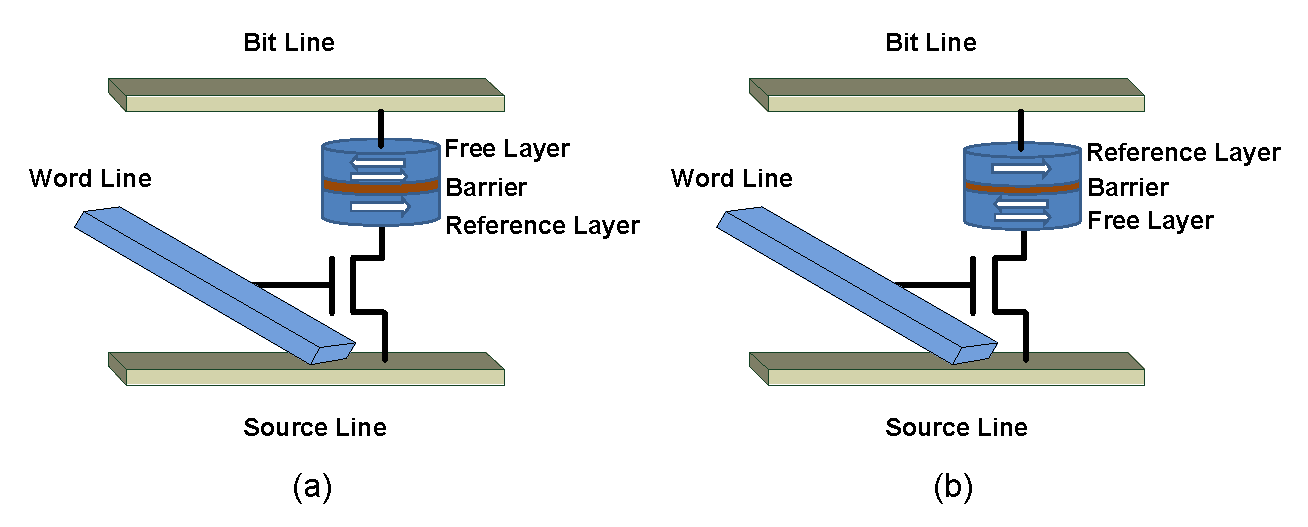
\includegraphics[width=3.5in]{fig/sttramcell.eps}
  \caption{Demonstration of a STT-RAM cell: (a) Conventional connection scheme; (b) Reverse connection scheme.}
  \label{fig:sttcell}
\end{figure}

Another important metric for an MTJ is the tunnel magnetoresistance~(TMR) which is defined as,
\begin{equation}
TMR = \frac{R_{AP}-R_{P}}{R_{P}}
\label{eqn:tmr}
\end{equation}
where ${R_{AP}}$ is the electrical resistance in the anti-parallel state, whereas ${R_{P}}$ is the resistance in the parallel state. A large TMR means big gap between low resistance state~(LRS) and high resistance state~(HRS), which could essentially brings faster read sensing latency or relaxes the constraint for sense amplifier design. It's critical to introduce an equivalent metric for a STT-RAM cell which contains both the MTJ and the access transistor. Similarly the cell TMR~(CTMR) is defined as,
\begin{equation}
CTMR = \frac{R_{cell,AP}-R_{cell,P}}{R_{cell,P}}
\label{eqn:ctmr}
\end{equation}
where $R_{cell,AP}$ is the total cell resistance when the MTJ is in the anti-parallel state, whereas $R_{cell,P}$ is the total cell resistance when the MTJ is in the parallel state. CTMR can be expressed by another equation,
\begin{equation}
CTMR = \frac{I_{P}-I_{AP}}{I_{AP}}
\label{eqn:ctmr2}
\end{equation}
where ${I_{AP}}$ and ${I_{P}}$ are the currents for reading ``0" state and ``1" state. If we ignore the resistance difference of the access transistor for reading ``0" state and ``1" state. CTMR can be interpreted as,
\begin{equation}
CTMR = \frac{R_{AP}-R_{P}}{R_{P}+R_{NMOS}} = \frac{R_{AP}-R_{P}}{R_{P}+\frac{C}{W}}
\label{eqn:ctmr3}
\end{equation}
where $R_{NMOS}$ is the equvalent resistance of access NMOS transistor and $W$ is the transistor width, $C$ is a constant related to the wordline voltage and threshold voltage of the transistor. From equation~\ref{eqn:ctmr3} we can conclude that sizing up the access transistor will make CTMR close to the inherent TMR of MTJ.

\subsection{Write current versus write pulse width trade-off}
The current amplitude required to reverse the direction of the free ferromagnetic layer is determined by a lot of factors such as material property, device geometry and importantly the write pulse duration. Generally, the longer the write pulse is applied, the less the switching current is needed to switch the MTJ state. Three distinct switching modes were identified~\cite{STTRAM:JAP07} according to the operating range of switching pulse width $\tau$: thermal activation ($\tau>20ns$), processional switching ($\tau<3ns$) and dynamic reversal ($3ns<\tau<20ns$). 

\begin{figure}[t]
  \centering
  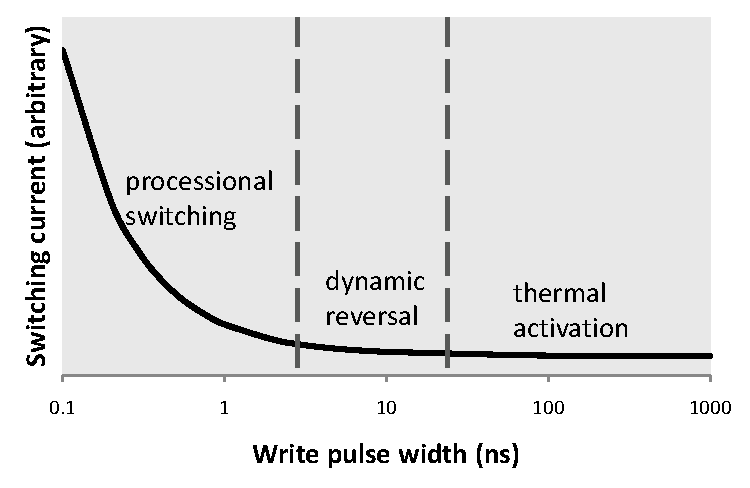
\includegraphics[width=3in]{fig/IcWt.eps}
  \caption{Demonstration of three switching phases: thermal activation, dynamic reversal and precessional switching.}
  \label{fig:IcWt}
\end{figure}

The relationship between switching current current $J_{c}$ and write pulse width $\tau$ was characterized by an analytical model in~\cite{STTRAM:IEDM09}. The equations are listed as follows,
\begin{eqnarray}
J_{c,TA}(\tau) &=& J_{c0}\{1- (\frac{k_{B}T}{E_{b}})ln(\frac{\tau}{\tau_{0}})\} \label{eqn:jcta} \\
J_{c,PS}(\tau) &=& J_{c0}+ \frac{C}{\tau^{\gamma}} \label{eqn:jcps} \\
J_{c,DR}(\tau) &=& \frac{J_{c,TA}(\tau)+J_{c,PS}(\tau)e^{-k(\tau - \tau_{c})}}{1+e^{-k(\tau - \tau_{c})}} \label{eqn:jcdr} 
\end{eqnarray}  
where $J_{c,TA}$, $J_{c,PS}$, $J_{c,DR}$ are the switching current density for thermal activation, precessional switching and dynamic reversal. $J_{c0}$ is the critical switching current density. $k_{B}$ is the Boltzmann constant, $T$ is the temperature, $E_{b}$ is the thermal barrier, and $\tau_{0}$ is inverse of the attempt frequency. $C$, $\gamma$, $k$, and $\tau_{c}$ are fitting constants. Based on the observation from Figure~\ref{fig:IcWt} and analysis of the analytical model,  we found very different switching characteristics in the three switching modes. For example, in thermal activation mode, the required switching current decrease very slowly even we increase the write pulse width by orders of magnitude, thus short write pulse width is more favorable in this regime because reducing write pulse can reduce both write latency and energy without much penalty on read latency and energy. While in processional switching, write current goes up rapidly if we further reduce write pulse width, therefore minimum write energy of the MTJ is achieved at some particular write pulse width in this regime. Consequently, this paper will focus on the exploration of write pulse width in processional switching and dynamic reversal to optimize for different design goals.

\subsection{Perpendicular MTJ}

\section{STT-RAM Macro Modeling} \label{sec:model}

\subsection{Area Modeling}
To simulate the performance of a single STT-RAM cell, it is important to estimate its access area first. As mentioned before, each 1T1J STT-RAM cell is composed of one NMOS and one MTJ. The NMOS access device is connected in series with the MTJ as shown in Figure~\ref{fig:1t1r}. The size of NMOS is constrained by both $I_{c}(AP\rightarrow P)$ and $I_{c}(P\rightarrow AP)$, which are inversely proportional to the writing pulse width. In order to estimate the current driving ability of MOSFET devices, a small test circuit using HSPICE with PTM 45nm HP model~\cite{PTM} is simulated. The BL-to-SL current and SL-to-BL current are obtained by assuming typical TMR (120\%) and LRS ($3k\Omega$) value~\cite{STTRAM:Qualcomm09} and bursting wordline voltage to be 1.5V (the optimal $V_{WL}$ value is extracted from~\cite{STTRAM:Gatech10}). As we can see in Figure~\ref{fig:icw}, the SL-to-BL current is always smaller and saturate faster than BL-to-SL current. Such current degradation is related to the body effect of the access transistor, where the threshold voltage is boosted by a positive source-to-substrate voltage different $V_{SB}=I_{c}\times R$ ($I_{c}$ is the current passing through MTJ and $R$ is the resistance of the MTJ). Thus we always choose the connecting scheme which use BL-to-SL current to match the maximum of $I_{c}(AP\rightarrow P)$ and $I_{c}(P\rightarrow AP)$ and SL-to-BL to match the minimum of them. The corresponding access transistor width must satisfy the following conditions,
\begin{eqnarray}
I_{BS}(W_{BS}) &\geq& max(I_{c}(AP\rightarrow P), I_{c}(P\rightarrow AP)) \\
I_{SB}(W_{SB}) &\geq& min(I_{c}(AP\rightarrow P), I_{c}(P\rightarrow AP))
\end{eqnarray}
where $I_{BS}(W_{BS})$ is the current from BL to SL with transistor width $W_{BS}$ and $I_{SB}(W_{SB})$ is the current from SL to BL with transistor width $W_{SB}$.

\begin{figure}[t]
  \centering
  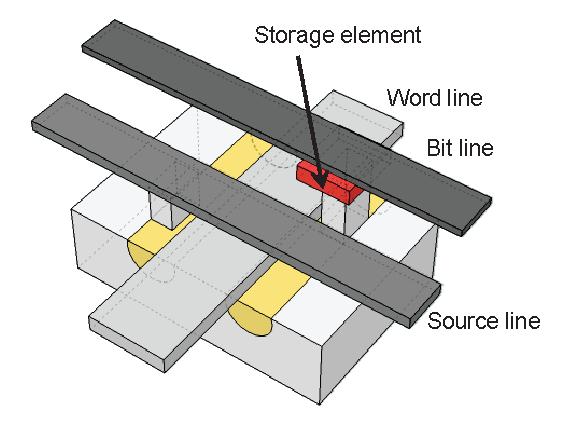
\includegraphics[width=2.5in]{fig/1t1r.eps}
  \caption{Conceptual view of a MOS-accessed cell (1T1J) and its connected word line, bit line, and source line.}
  \label{fig:1t1r}
\end{figure}
\begin{figure}[t]
  \centering
  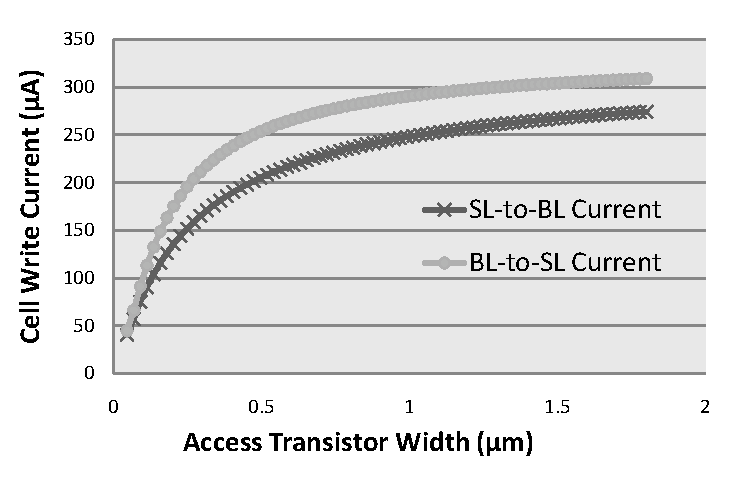
\includegraphics[width=2.5in]{fig/IC_W.eps}
  \caption{Driving ability of 45nm NMOS access transistor.}
  \label{fig:icw}
\end{figure}

The relationship between access transistor width and CTMR defined in Section~\ref{subsec:cell} was also simulated. As can be seen in Figure~{fig:cmtrw}, a larger access transistor increase CTRM closer to the inherent TRM value of MTJ. It's necessary to set a lower bound $CTMR_{min}$ for CTMR to guarantee the correctness of read operation. Thus the transistor width must be large enough to satisfy the minimum CTMR requirement,
\begin{equation}
CTMR(W_{CTMR}) \geq CTMR_{min}
\end{equation}
Finally we will choose a transistor width $W$ which satisfy all the above requirements,
\begin{equation}
W = max(W_{BS}, W_{SB}, W_{CTMR}) \label{equ:width}
\end{equation}

\begin{figure}[t]
  \centering
  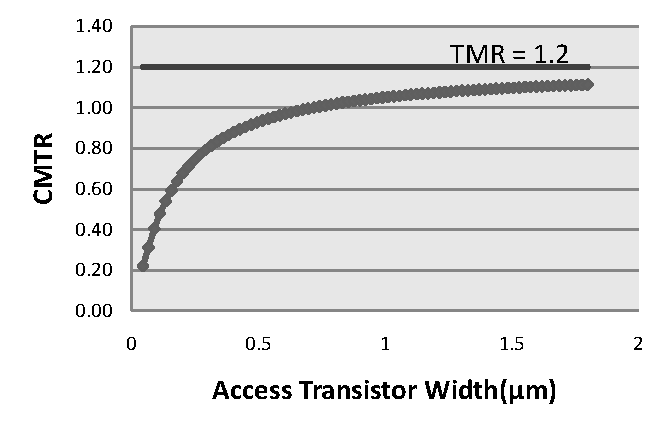
\includegraphics[width=2.6in]{fig/CMTR_W.eps}
  \caption{Cell MTR versus transistor width.}
  \label{fig:cmtrw}
\end{figure}

To achieve high cell density, we model the STT-RAM cell area by referring to DRAM design rules~\cite{DRAM:6F2}.  As a result, the cell size of a STT-RAM cell is calculated as follows,
\begin{equation}
\mathrm{Area}_{\mathrm{cell}}={3\left(W/L+1\right)}(F^2)
\end{equation}

\subsection{Data sensing modeling}
Three sensing modes were proposed in~\cite{CACTI:DATE11:Xu} to sense resistance-based NVMs including STT-RAM, PCRAM and ReRAM: current sensing, current-in voltage sensing, and voltage-divider sensing. There are trade-offs between the area, latency and energy of the three sensing modes. For example, current sensing is the fastest approach~\cite{RRAM:ITRI11} to sense the state if the number of cells per bitline is larger than 64, while voltage-divider sensing the second fastest and the current-in voltage sensing is slowest. In contrast, current-in voltage sensing has the best area efficiency which is defined as the ratio of NVM cell area to the prototype area while current-in sensing has the worst area efficiency. In this work, we will focus on current sensing scheme to reduce read latency. We adapt the current-voltage converter and sense amplifier design discussed in~\cite{CACTI:DAC08:Dong}. The current-voltage converter in our current sensing scheme is actually the first-level sense amplifier, and the conventional voltage sense amplifier is still kept as the final stage of the sensing scheme. In order to maintain low rate of read disturbance, it's necessary to reduce read current when choosing longer write pulse and smaller write current. And reduced read current have impact on the latency of current-voltage converter and sense amplifier. Therefore We use HSPICE to simulate the latency, energy and leakage of the two-stage sense amplifier with different read current and build a look-up table in NVsim.

\subsection{Cell Switching Modeling}
Dynamic MTJ switching model was developed in~\cite{STTRAM:Purdue10} with consideration of the switching phenomenon involves magnetoresistive effects, which can not estimated only by RC analysis.  However, this work is focusing on static analysis of STT-RAM and NVSim does not model the dynamic behavior during the switching of the cell state. Thus we use simply calculate switching energy (i.e. cell write energy) by using Joule's first law that is,
\begin{equation}
\mathrm{Energy}_{\mathrm{cell_switching}} = I_{c}^2 R \tau \label{equ:cellenergy}
\end{equation}
in which the resistance value $R$ can be the equivalent resistance of the corresponding LRS or HRS (i.e. $R_{P}$ or $R_{AP}$). Taking the switching current versus switching pulse width as input for Equation~\ref{equ:cellenergy}, we can easily get the relation between the energy of switching one cell and write pulse width. It can been seen in Figure~\ref{fig:cellenergy}, minimum switching energy per cell is achieved at write pulse width $\tau_{min_cell_energy}$ in the range of processional switching mode. However, the the optimal operating write pulse width from cell-level point of view is not necessarily the best operating point from system-level point of view because the effect of access transistor and peripheral circuitry have not been considered.
\begin{figure}[t]
  \centering
  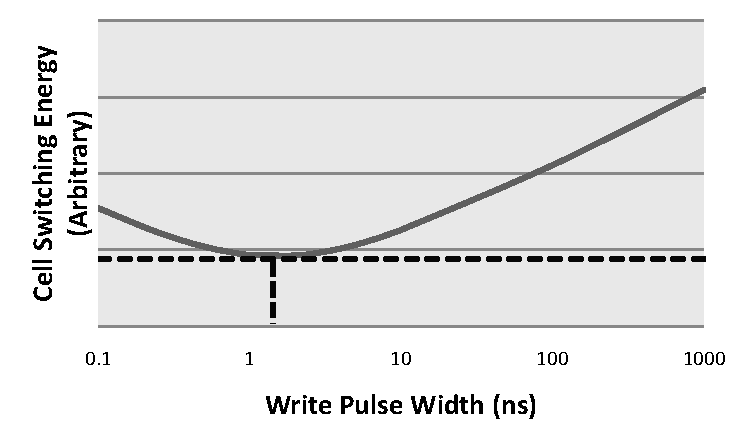
\includegraphics[width=2.5in]{fig/cellenergy.eps}
  \caption{Switching energy per cell versus write pulse width.}
  \label{fig:cellenergy}
\end{figure}


\section{STT-RAM Cache Design Optimization} \label{sec:opt}

\begin{figure}[t]
  \centering
  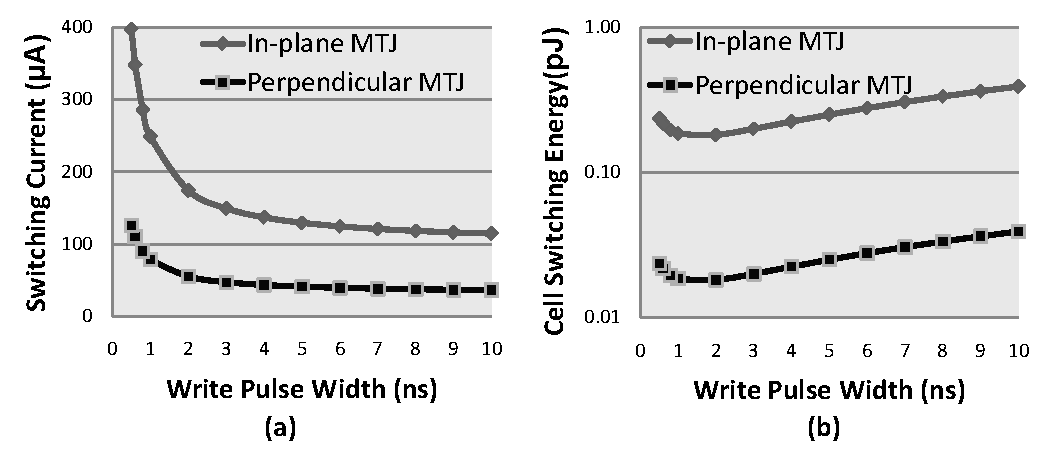
\includegraphics[width=3.5in]{fig/MTJSpec.eps}
  \caption{Representative data curves of in-plane and perpendicular MTJs: (a)Switching current; (b) Cell switching energy.}
  \label{fig:specs}
\end{figure}

\begin{figure*}[t]
  \centering
  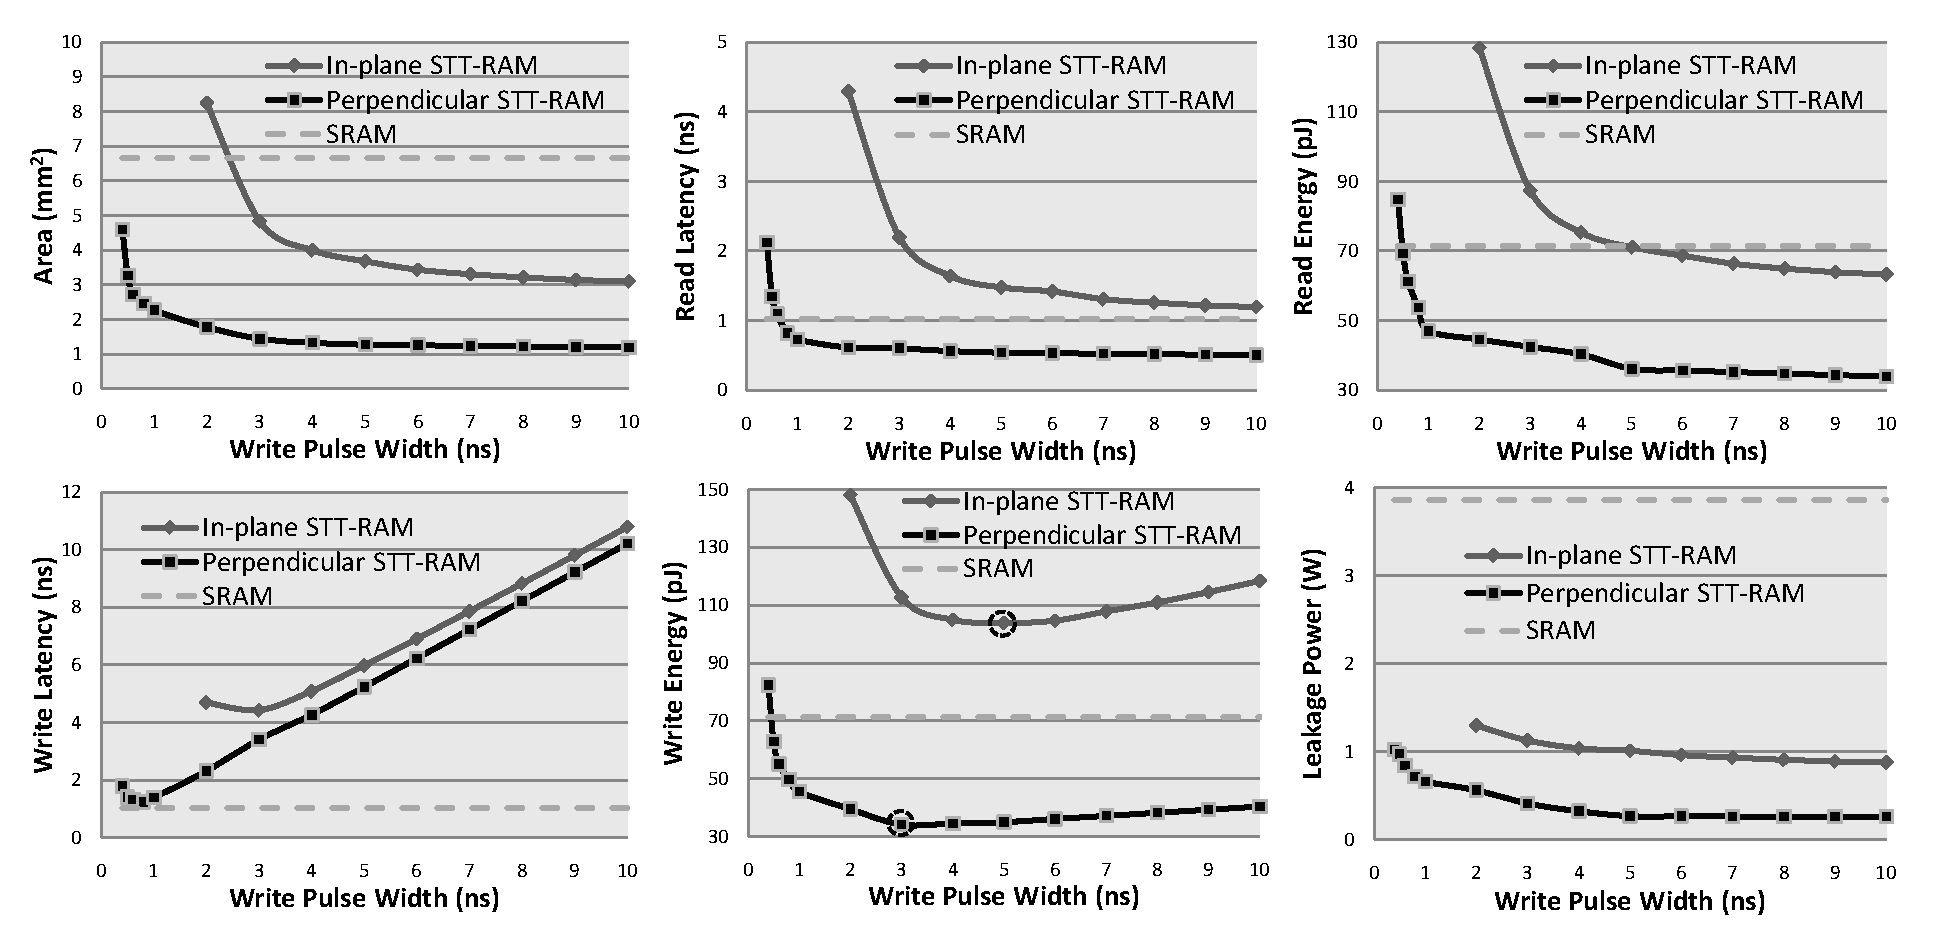
\includegraphics[width=7in]{fig/AllMetrics.eps}
  \caption{Metrics of SRAM and STT-RAM built with in-plane and perpendicular MTJs: (a)Area; (b)Read latency; (c)Read energy; (d)Write latency; (e)Write energy; (f)Leakage power.}
  \label{fig:metrics}
\end{figure*}

\begin{figure}[t]
  \centering
  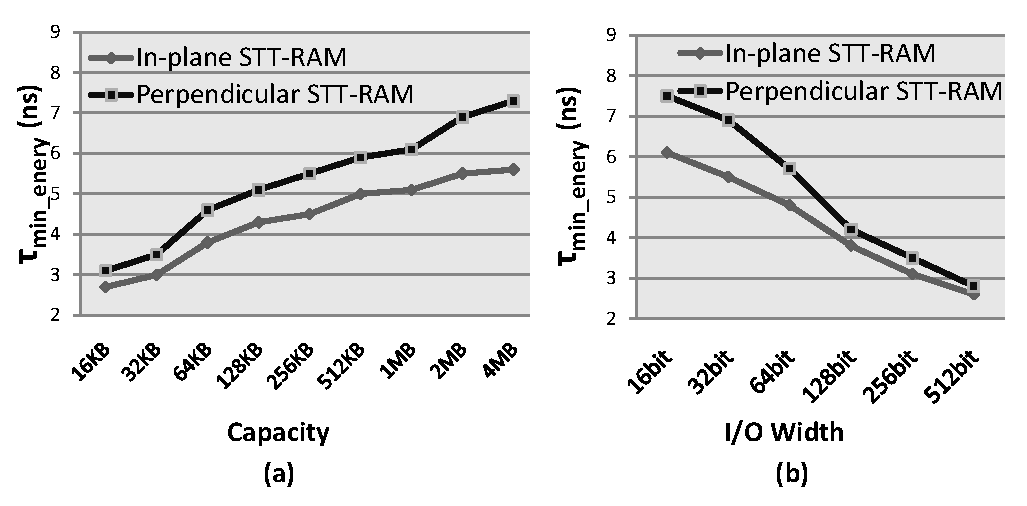
\includegraphics[width=3in]{fig/MinEnergy.eps}
  \caption{Dependence of $\tau_{min\_energy}$ on STT-RAM Macro Capacity.}
  \label{fig:minenergy}
\end{figure}
\section{Case Study} \label{sec:case}
In this section we will conduct one case study to demonstrate how the device-architecture co-optimization methodology can help design STT-RAM cache with different optimization directions. We will replace the L1 SRAM instruction cache and data cache by there different STT-RAM caches: latency-optimized STT-RAM, energy-optimized STT-RAM, or EDP-optimized STT-RAM. We are the first to explore design space of STT-RAM utilizing PMTJ as L1 cache replacement and compare the results with The optimization techniques are the same with those used in Section~\ref{subsec:co-opt}.

\subsection{Experimental Setup}

DIMIN, PUT YOUR STUFF HERE.

\begin{table}[t]
\centering
\caption{Simulation Parameters}
\label{tb:parameters}
\vspace{-5pt}
\begin{tabular}{ l | c }
\hline \hline
Components & Features\\
\hline
Simulator kernel & SystemC 2.2.0\\
\hline
CPU core & ARM9TDMI and XScale compatible \\
\hline
\multirow{2}{*}{Cache configurations} & 4-way associative 16K L1 cache  \\
& 4B cache line size \\
\hline
\multirow{2}{*}{Bus} & 32-bit address bus  \\
& 32-bit data bus \\
\hline
Clock frequency & $1GHz$ \\
\hline
Main memory & 64MB DRAM \\
\hline
Benchmark & MiBench \\
\hline\hline
\end{tabular}
\vspace{-10pt}
\end{table}

\subsection{Experimental Results}

\begin{figure}[t]
\centering
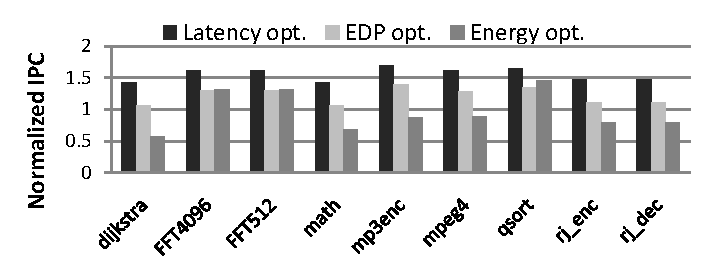
\includegraphics[width=0.4\textwidth]{fig/IPC}
\vspace{-10pt}
\caption{Normalized IPC for STT-RAM with different optimization directions.}
\label{fig:ipc}
\vspace{7pt}
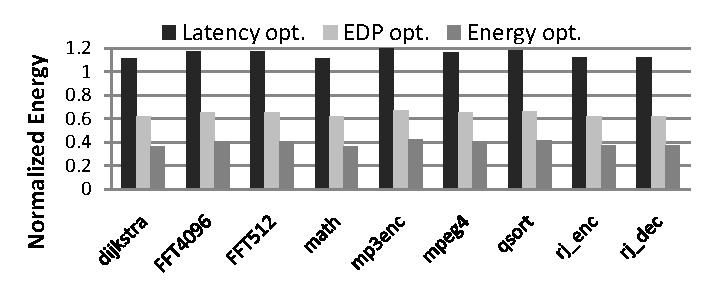
\includegraphics[width=0.4\textwidth]{fig/Energy}
\vspace{-10pt}
\caption{Normalized energy for STT-RAM with different optimization directions.}
\label{fig:energy}
\vspace{7pt}
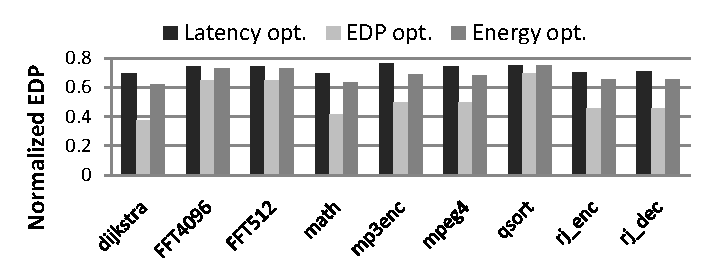
\includegraphics[width=0.4\textwidth]{fig/EDP}
\vspace{-10pt}
\caption{Normalized EDP for STT-RAM with different optimization directions.}
\label{fig:edp}
\vspace{-10pt}
\end{figure}

\begin{figure}[t]
  \centering
  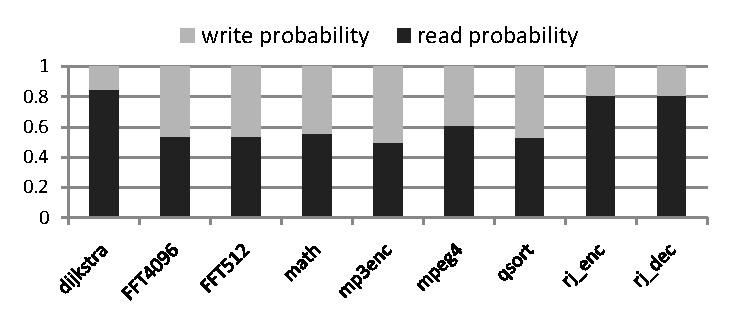
\includegraphics[width=2.8in]{fig/RWratio.eps}
%  \vspace{-10pt}
  \caption{Read-write ratio for different benchmarks.}
  \label{fig:ratio}
\vspace{-15pt}
\end{figure} 

We normalize instruction per cycle (IPC), energy and EDP to SRAM-based cache. Note that energy here includes read dynamic energy, write dynamic energy and leakage energy. Figure~\ref{fig:ipc} shows the simulations results in terms of normalized IPC when using the three different STT-RAM caches. Figure~\ref{fig:energy} presents the energy saving percentage of replacing SRAM by these STT-RAM caches. Figure~\ref{fig:edp} illustrates the EDP value of STT-RAM caches for different benchmarks. We can see that the latency-optimized STT-RAM has almost 50\% better IPC than SRAM, while it has negative energy saving compared to SRAM. Energy-optimized STT-RAM has approximately 60\% average energy saving compared to SRAM while maintaining only 8\% degraded IPC of SRAM. EDP-optimized STT-RAM has about 20\% better IPC than SRAM and also nearly 40\% energy saving compared to SRAM. Figure~\ref{fig:ratio} shows the variation in read/write statistics for different benchmarks. 
\section{Conclusion} \label{sec:conclusion}

In this paper, we analyze the impact of write pulse width on area, performance, and energy of STT-RAM array and develop a methodology for device-architecture co-design of STT-RAM based caches with different optimization goals. We take both near-commercialized in-plane MTJ and advanced PMTJ as optimization targets. Our study shows that for a given MTJ spec the quality of STT-RAM macro strongly depends on the write pulse width. In general, reducing write pulse width will harm area, read operation and leakage and these metrics were exacerbated when the write pulse is shorter than some certain width in processional mode. While write latency/energy is not a non-monotonic function of write pulse width. Therefore it's important to find the optimal write pulse width for minimum write latency or energy. We combine the write pulse width optimization with other architectural techniques to design STT-RAM macro as DRAM or SRAM replacement. A $64MB$ STT-RAM chip design spectrum was demonstrated as potential replacement in low power embedded system. Three STT-RAM caches are verified as L1 cache replacement in an embedded system and the simulation results show that by utilizing advanced PMTJ STT-RAM based L1 cache can outperform SRAM in system performance and energy separately or even simultaneously. 

\bibliographystyle{IEEEtran}
\bibliography{bib/cacti,bib/mram,bib/spintronic,bib/sttram}

\end{document} 